% Relatório técnico — Projeto Final de Sistemas Operacionais (UniSENAC)
% Compile com pdfLaTeX, duas vezes (por causa do sumário): pdflatex relatorio.tex
% No Overleaf: suba esta pasta inteira (relatorio.tex e figuras/) e use o compilador pdfLaTeX.
% Trechos marcados com \pendente{...} ainda precisam ser preenchidos pelo grupo.

\documentclass[12pt,a4paper]{article}

\usepackage[T1]{fontenc}
\usepackage[utf8]{inputenc}
\usepackage[brazil]{babel}
\usepackage{lmodern}
\usepackage[a4paper,top=3cm,left=3cm,bottom=2cm,right=2cm]{geometry}
\usepackage{setspace}
\usepackage{indentfirst}
\usepackage{graphicx}
\usepackage{booktabs}
\usepackage{tabularx}
\usepackage{xcolor}
\usepackage{listings}
\usepackage{float}
\usepackage{hyperref}

\onehalfspacing
\setlength{\parindent}{1.25cm}
\hypersetup{colorlinks=true, linkcolor=black, urlcolor=blue!60!black, citecolor=black}

% Marca de pendência: descomente o \renewcommand para ela sumir do PDF final.
\newcommand{\pendente}[1]{\textcolor{red}{\textbf{[PENDENTE:} #1\textbf{]}}}
% \renewcommand{\pendente}[1]{}

\lstset{
  basicstyle=\ttfamily\small,
  breaklines=true,
  frame=single,
  columns=fullflexible,
  keepspaces=true,
  showstringspaces=false,
  literate={á}{{\'a}}1 {à}{{\`a}}1 {ã}{{\~a}}1 {â}{{\^a}}1 {é}{{\'e}}1 {ê}{{\^e}}1 {í}{{\'i}}1
           {ó}{{\'o}}1 {õ}{{\~o}}1 {ô}{{\^o}}1 {ú}{{\'u}}1 {ç}{{\c{c}}}1
}

\newcommand{\titulo}{Transcritor: transcrição de áudio local com processos, semáforo e escalonamento}
\newcommand{\professor}{\pendente{nome do professor}}

\begin{document}

% ========== CAPA ==========
\begin{titlepage}
  \centering
  {\large\textbf{Centro Universitário SENAC -- UniSENAC}}\\[0.3cm]
  {\large Análise e Desenvolvimento de Sistemas}\\[0.3cm]
  {\large Sistemas Operacionais}\\[3cm]
  {\large
    \pendente{Integrante 1}\\
    \pendente{Integrante 2}\\
    \pendente{Integrante 3}\\
    \pendente{Integrante 4}\\
  }
  \vfill
  {\LARGE\textbf{\titulo}}\\[0.8cm]
  {\large Relatório Técnico do Projeto Final}\\[0.5cm]
  {\large Professor(a): \professor}
  \vfill
  {\large Porto Alegre}\\
  {\large 2026}
\end{titlepage}

\tableofcontents
\newpage

% ========== 1. TEMA E DESCRIÇÃO ==========
\section{Tema e descrição do projeto}

O Transcritor é um aplicativo de transcrição de áudio e vídeo que roda no computador de
quem o usa. O público são profissionais que trabalham com entrevistas gravadas, principalmente
jornalistas: a pessoa arrasta os arquivos para a página, escolhe o idioma e recebe o texto
com a marcação de tempo de cada fala, em TXT ou em SRT (legenda).

Por rodar na própria máquina, a gravação nunca sai do computador. Isso importa para
jornalistas, que lidam com fontes e material sigiloso. O custo dessa escolha é que o
aplicativo precisa se adaptar ao hardware que encontrar: um notebook sem placa de vídeo, um
desktop com GPU NVIDIA, Linux, Windows ou Mac. Por isso, na primeira execução, o próprio
aplicativo lê o sistema operacional, os núcleos, a memória RAM e a placa de vídeo, mostra
quais modelos de reconhecimento de fala cabem naquela máquina, baixa o recomendado e passa a
transcrever na GPU, se houver, ou na CPU.

A transcrição é feita pelo modelo Whisper~\cite{whisper}, que é pesado: um áudio de uma hora
ocupa a máquina por minutos. Para atender vários arquivos ao mesmo tempo sem travar a
interface, o aplicativo é dividido em um processo principal, que recebe os pedidos e
organiza a fila, e vários processos \emph{worker}, que fazem a transcrição. É nessa divisão que
aparecem os conceitos de Sistemas Operacionais do trabalho: criação de processos,
comunicação entre processos, threads, exclusão mútua, semáforo, escalonamento,
tratamento de falhas, sinais e gerência de memória (Figura~\ref{fig:arquitetura}).

\begin{figure}[H]
  \centering
  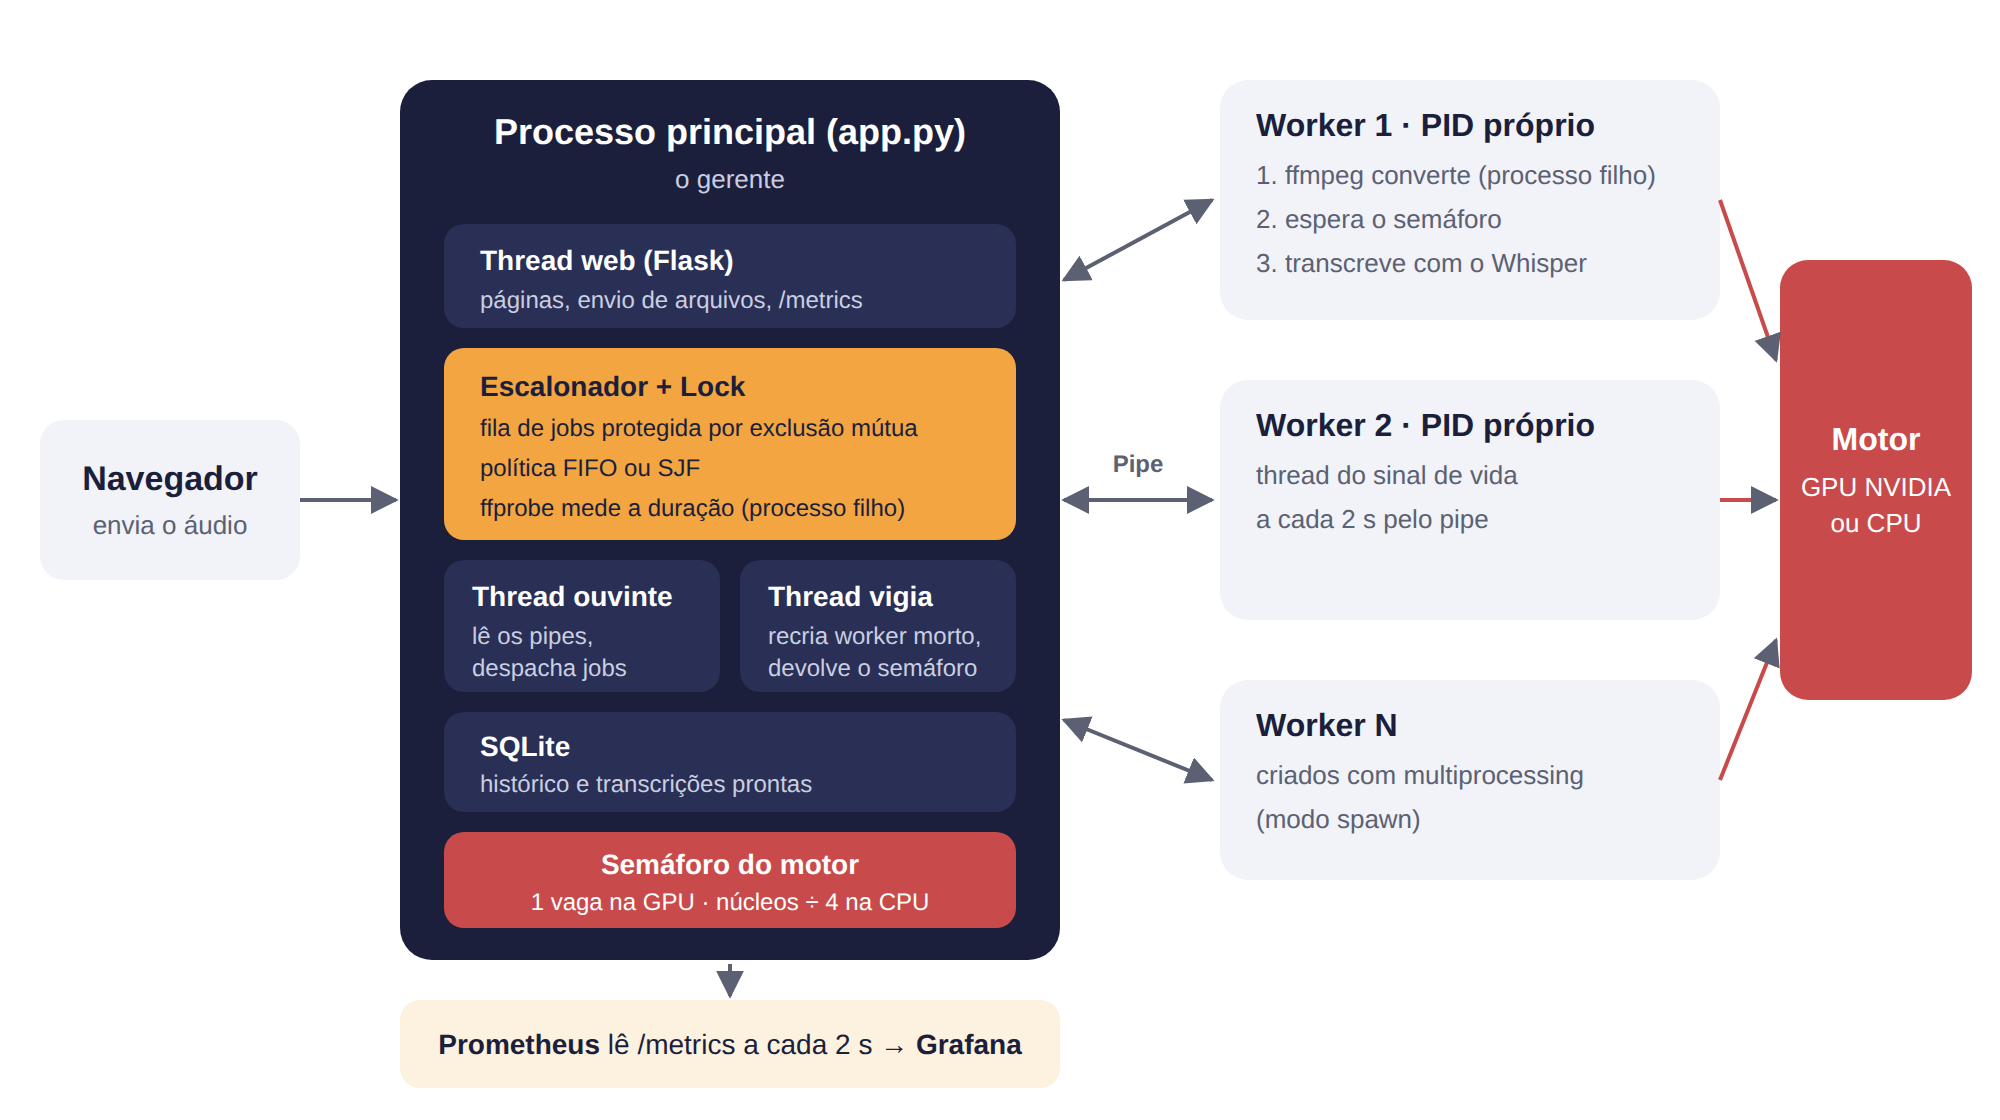
\includegraphics[width=\textwidth]{figuras/arquitetura.png}
  \caption{Arquitetura do Transcritor}
  \label{fig:arquitetura}
\end{figure}

% ========== 2. OBJETIVO ==========
\section{Objetivo}

\subsection{Objetivo geral}
Desenvolver um aplicativo de transcrição de áudio e vídeo que funcione em qualquer
computador, com ou sem placa de vídeo, e que mostre, de forma observável, como o sistema
operacional cria, sincroniza, escalona e recupera processos durante a execução de uma
aplicação real.

\subsection{Objetivos específicos}
\begin{itemize}
  \item Detectar o hardware da máquina e oferecer só os modelos que cabem nela;
  \item Transcrever vários arquivos em paralelo com processos \emph{worker} independentes;
  \item Garantir, com um semáforo, que a GPU seja usada por um processo de cada vez;
  \item Permitir trocar a política de escalonamento (FIFO ou SJF) com o aplicativo rodando;
  \item Recuperar o trabalho de um \emph{worker} que morra no meio da transcrição;
  \item Mostrar processos, fila, semáforo e uso de CPU e memória num painel do Grafana;
  \item Oferecer scripts que demonstrem cada conceito em poucos segundos.
\end{itemize}

% ========== 3. METODOLOGIA ==========
\section{Metodologia}

\pendente{Como o grupo trabalhou: divisão de tarefas entre os quatro integrantes, reuniões,
uso do Git e do GitHub.}

O código fica num repositório público no GitHub, com testes automáticos executados a cada
envio (GitHub Actions). O desenvolvimento e os testes foram feitos no Linux, com Docker e
direto no sistema, numa máquina com GPU NVIDIA RTX 4060 (8 GB) e em modo só CPU.
\pendente{Testar no Windows e registrar aqui.}

\subsection{Funcionalidades implementadas}
\begin{itemize}
  \item Detecção do sistema: sistema operacional, arquitetura, núcleos, RAM e GPU NVIDIA com sua VRAM;
  \item Catálogo de seis modelos (de \emph{Tiny} a \emph{Large v3}), marcando os que cabem e o recomendado;
  \item Instalação automática do modelo recomendado na primeira execução, e dos outros com um clique;
  \item Envio de vários arquivos de áudio ou vídeo de uma vez, arrastando para a página;
  \item Escolha do idioma ou detecção automática;
  \item Fila com acompanhamento ao vivo: situação, progresso e qual \emph{worker} (e PID) está em cada arquivo;
  \item Visualização do texto com marcação de tempo e exportação em TXT e SRT;
  \item Troca da política de escalonamento (FIFO ou SJF) pela página;
  \item Botão para matar um \emph{worker}, usado na demonstração de tolerância a falhas;
  \item Métricas para o Prometheus e painel pronto no Grafana;
  \item Scripts de demonstração de concorrência, falha e escalonamento.
\end{itemize}

\begin{figure}[H]
  \centering
  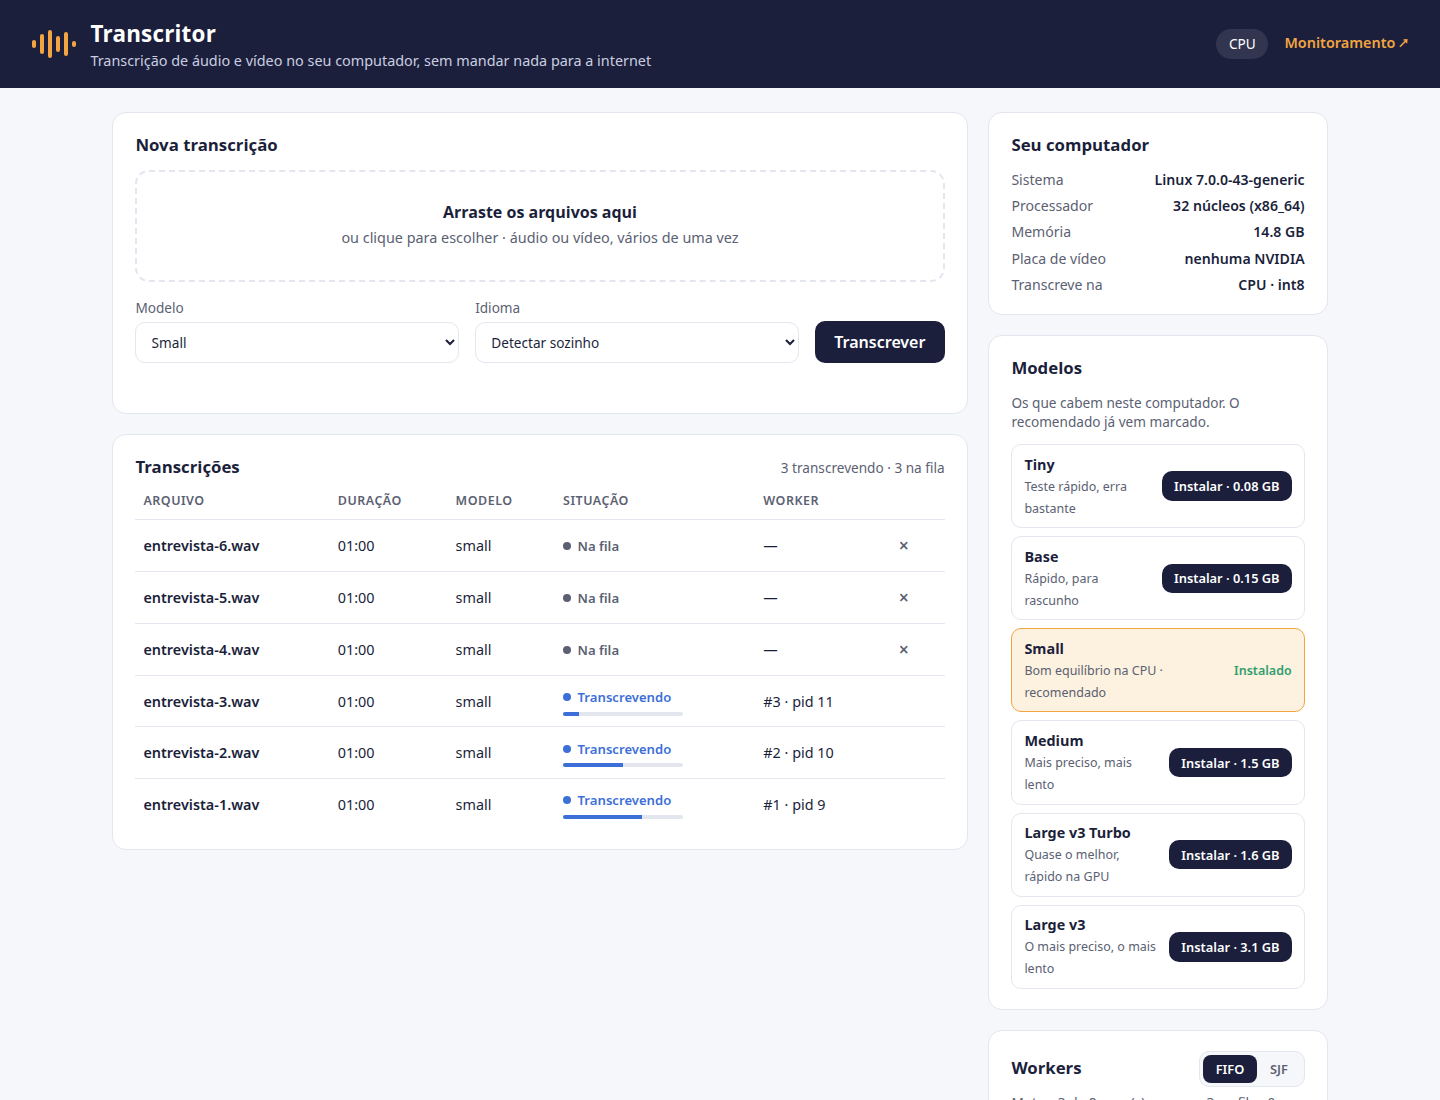
\includegraphics[width=\textwidth]{figuras/app.png}
  \caption{Tela do Transcritor transcrevendo seis arquivos com três \emph{workers}}
  \label{fig:app}
\end{figure}

\subsection{Tecnologias utilizadas}

\begin{table}[H]
\centering
\begin{tabularx}{\textwidth}{@{}lX@{}}
\toprule
\textbf{Camada} & \textbf{Tecnologia} \\
\midrule
Execução & Docker e Docker Compose; ou Python direto no sistema \\
Aceleração & NVIDIA CUDA 12 e cuDNN 9 (opcional) \\
Áudio e vídeo & FFmpeg e FFprobe \\
Monitoramento & Prometheus e Grafana \\
Testes & pytest e GitHub Actions \\
\bottomrule
\end{tabularx}
\caption{Tecnologias do projeto}
\end{table}

\subsection{Linguagem de programação}
\textbf{Python 3.12} no aplicativo e nos scripts de demonstração. A página usa HTML, CSS e
JavaScript, sem \emph{framework}.

\subsection{Banco de dados}
\textbf{SQLite}, num arquivo dentro da pasta de dados. Ele guarda cada transcrição: nome do
arquivo, duração, modelo, situação, \emph{worker} e PID que a fez, tentativas, horários e o
texto com os tempos. Só o processo principal acessa o banco, com uma trava (\texttt{Lock})
porque as threads dele escrevem ao mesmo tempo. Se o aplicativo for fechado com arquivos na
fila, eles voltam para a fila na próxima execução.

\subsection{Frameworks}
\begin{itemize}
  \item \textbf{Flask}: servidor web e API;
  \item \textbf{faster-whisper} sobre \textbf{CTranslate2}: execução do modelo Whisper na GPU ou na CPU.
\end{itemize}

\subsection{Bibliotecas}
\begin{itemize}
  \item \texttt{multiprocessing}, \texttt{threading} e \texttt{subprocess} (da biblioteca padrão):
        processos, \emph{pipes}, semáforo, travas, threads e processos filhos;
  \item \texttt{sqlite3} (da biblioteca padrão): banco de dados;
  \item \texttt{psutil}: memória total da máquina e CPU e memória de cada \emph{worker};
  \item \texttt{prometheus-client}: exposição das métricas em \texttt{/metrics};
  \item \texttt{av} (PyAV): leitura do áudio pelo faster-whisper;
  \item \texttt{nvidia-cublas-cu12} e \texttt{nvidia-cudnn-cu12}: bibliotecas da CUDA, só para GPU.
\end{itemize}

% ========== 4. CONCEITOS DE SO ==========
\section{Conceitos de Sistemas Operacionais aplicados}

\subsection{Processos}
Cada \emph{worker} é um processo do sistema operacional, criado com
\texttt{multiprocessing.Process} no modo \texttt{spawn}, que inicia um interpretador Python
novo. Esse é o modo padrão do Windows e do macOS, e foi usado também no Linux para que o
programa se comporte igual nos três. Cada \emph{worker} tem seu PID, sua memória e seu
próprio modelo carregado; se um deles travar ou morrer, os outros e a página continuam.

Os processos passam pelos estados vistos em aula~\cite{tanenbaum}: o \emph{worker} fica
\emph{bloqueado} esperando um trabalho no \emph{pipe} ou esperando o semáforo, fica
\emph{executando} enquanto converte ou transcreve, e termina quando recebe o aviso de
encerramento. O painel do Grafana mostra essa linha do tempo para cada processo
(Figura~\ref{fig:grafana}).

\begin{lstlisting}[language=Python]
processo = self.contexto.Process(target=worker.executar, name=f"worker-{numero}",
                                 args=(numero, conexao_do_worker, self.semaforo, self.ajustes))
processo.start()
\end{lstlisting}

\subsection{Processos filhos}
O processo principal chama o \texttt{ffprobe} para medir a duração de cada arquivo, e o
\emph{worker} chama o \texttt{ffmpeg} para converter o áudio para o formato do modelo (16 kHz,
mono). Os dois são programas externos, executados como processos filhos com
\texttt{subprocess.run}, que cria o processo e espera ele terminar.

\subsection{Comunicação entre processos}
Processos não compartilham memória, então o gerente e cada \emph{worker} conversam por um
\texttt{Pipe}, um canal de mão dupla oferecido pelo sistema operacional. O gerente manda o
trabalho; o \emph{worker} devolve mensagens: \texttt{livre}, \texttt{estado},
\texttt{progresso}, \texttt{fim}, \texttt{erro} e \texttt{vivo}. Usar um \emph{pipe} por
\emph{worker}, e não uma fila única, tem um motivo: se um processo morrer no meio de uma
escrita, só o canal dele fica corrompido, e ele é descartado junto com o processo.

A thread ouvinte do gerente espera em todos os \emph{pipes} ao mesmo tempo com
\texttt{multiprocessing.connection.wait}, que fica bloqueada até algum deles ter dados.

\subsection{Threads e exclusão mútua}
O processo principal tem três threads: a do Flask, que atende a página; a ouvinte, que lê os
\emph{pipes} e entrega trabalhos; e a vigia, que confere os \emph{workers} a cada segundo. As
três mexem na mesma fila e na mesma lista de \emph{workers}. Sem proteção, duas threads
poderiam entregar o mesmo trabalho a dois \emph{workers}. Por isso, todo acesso a esses dados
fica dentro de uma seção crítica protegida por um \texttt{threading.Lock}:

\begin{lstlisting}[language=Python]
def adicionar(self, jobs):
    with self.trava:
        for job in jobs:
            self.escalonador.adicionar(job)
        self.despachar()
\end{lstlisting}

O mesmo acontece dentro do \emph{worker}: a thread do sinal de vida e a thread principal
escrevem no mesmo \emph{pipe}, então cada envio também passa por uma trava.

\subsection{Semáforo}
A GPU tem memória limitada: na RTX 4060 usada nos testes, o \emph{worker} que transcreve com
o modelo \emph{Large v3 Turbo} chega a cerca de 1,35 GB de VRAM, e volta a cerca de 100 MB
(só o contexto da CUDA) quando solta o modelo. Se três \emph{workers} carregassem o modelo ao mesmo tempo, a memória
poderia acabar. O acesso ao motor de transcrição é então controlado por um
\texttt{BoundedSemaphore} compartilhado entre os processos, com uma vaga na GPU. Na CPU, o
número de vagas é o de núcleos dividido por quatro, porque cada \emph{worker} usa quatro
threads de cálculo.

\begin{lstlisting}[language=Python]
canal.enviar("estado", job["id"], "esperando")
with semaforo:
    canal.enviar("estado", job["id"], "transcrevendo")
    modelo = motor.carregar(...)
    trechos, idioma = motor.transcrever(...)
    del modelo
\end{lstlisting}

Enquanto um \emph{worker} transcreve, os outros podem converter o próximo áudio com o
\texttt{ffmpeg}, que não usa a GPU, e ficam bloqueados no semáforo até a vez deles. O modelo
é carregado ao entrar na seção crítica e liberado ao sair, devolvendo a memória.

\subsection{Escalonamento}
Quando um \emph{worker} fica livre, o gerente escolhe o próximo trabalho da fila. Há duas
políticas, que podem ser trocadas com o aplicativo rodando~\cite{silberschatz}:

\begin{itemize}
  \item \textbf{FIFO} (\emph{First In, First Out}): o primeiro que chegou é o primeiro atendido.
        É justa, mas sofre o \emph{efeito comboio}: áudios curtos esperam atrás dos longos.
  \item \textbf{SJF} (\emph{Shortest Job First}): o áudio mais curto primeiro. A duração é
        conhecida antes de começar (medida pelo \texttt{ffprobe}), o que torna o SJF
        aplicável aqui. Reduz o tempo médio de espera, mas um áudio longo pode esperar
        indefinidamente se não pararem de chegar curtos (\emph{inanição}).
\end{itemize}

\begin{lstlisting}[language=Python]
if self.politica == "sjf":
    escolhido = min(self.fila, key=lambda job: (job["duracao"], job["criado"]))
else:
    escolhido = min(self.fila, key=lambda job: job["criado"])
\end{lstlisting}

O script \texttt{demo/3\_escalonamento.py} envia, de uma vez, três áudios de 300 segundos
seguidos de cinco de 15 segundos, primeiro com FIFO e depois com SJF. Na GPU, com três
\emph{workers}, o resultado foi:

\begin{table}[H]
\centering
\begin{tabular}{@{}lrrr@{}}
\toprule
\textbf{Política} & \textbf{Espera dos curtos} & \textbf{Curtos prontos em} & \textbf{Lote inteiro} \\
\midrule
FIFO & 152,2 s & 191,5 s & 198,5 s \\
SJF  &   1,3 s &   6,1 s & 125,0 s \\
\bottomrule
\end{tabular}
\caption{FIFO contra SJF na GPU (médias dos cinco áudios curtos)}
\end{table}

Na CPU (32 núcleos, modelo \emph{Small}), com três áudios longos de 90 segundos, o padrão se
repetiu:

\begin{table}[H]
\centering
\begin{tabular}{@{}lrrr@{}}
\toprule
\textbf{Política} & \textbf{Espera dos curtos} & \textbf{Curtos prontos em} & \textbf{Lote inteiro} \\
\midrule
FIFO & 116,3 s & 122,3 s & 126,7 s \\
SJF  &   2,3 s &   7,8 s &  92,7 s \\
\bottomrule
\end{tabular}
\caption{FIFO contra SJF na CPU (médias dos cinco áudios curtos)}
\end{table}

Nos dois casos o SJF também terminou o lote inteiro antes: com os curtos na frente, os
\emph{workers} ficam ocupados por igual, em vez de dois ficarem parados esperando o último
áudio longo.

\subsection{Tolerância a falhas e sinais}
Cada \emph{worker} tem uma thread que manda um sinal de vida (\texttt{vivo}) a cada dois
segundos. A thread vigia do gerente confere a cada segundo se cada processo está vivo
(\texttt{is\_alive}) e se mandou sinal nos últimos 15 segundos. Se o processo morreu, ou se
travou e ficou calado, o gerente:

\begin{enumerate}
  \item encerra o processo travado com \texttt{SIGKILL} (\texttt{TerminateProcess} no Windows);
  \item devolve o semáforo em nome dele, se ele estava dentro do motor; sem isso, a vaga
        ficaria presa para sempre e todos os outros \emph{workers} ficariam bloqueados,
        num impasse (\emph{deadlock});
  \item põe o trabalho de volta na fila, até duas tentativas, para que um arquivo que derruba
        o \emph{worker} não fique num ciclo sem fim;
  \item cria um processo novo no lugar.
\end{enumerate}

No teste com \texttt{demo/2\_falha.py}, o \emph{worker} 1 foi morto no meio de um áudio de
10 minutos. O gerente registrou a morte com código $-9$ (\texttt{SIGKILL}), devolveu o
semáforo, recolocou o trabalho na fila e o \emph{worker} 2 o concluiu na segunda tentativa.

Os sinais também são usados no encerramento: o processo principal trata o \texttt{SIGTERM}
(enviado pelo \texttt{docker stop}, por exemplo) avisando cada \emph{worker} para terminar, e
os \emph{workers} ignoram o \texttt{SIGINT}, para que um \texttt{Ctrl+C} no terminal seja
tratado só pelo processo principal.

\subsection{Gerência de memória e dispositivos}
Na partida, o aplicativo consulta a memória com \texttt{psutil} e a GPU com o
\texttt{nvidia-smi}, e cruza com o catálogo de modelos. Na GPU, escolhe o tipo de cálculo
\texttt{int8\_float16} (pesos em 8 bits, cálculo em 16 bits), que usa cerca de metade da
memória do modelo original; na CPU, \texttt{int8}. Um modelo só é oferecido se cabe na VRAM
(GPU) ou na RAM (CPU). Durante a execução, o painel mostra a memória residente (RSS) de cada
\emph{worker} subindo ao carregar o modelo. Na GPU, a VRAM volta ao mínimo quando o modelo é
solto. Na CPU, a RAM do processo cai só em parte: a memória liberada pelo programa fica
reservada pelo alocador do processo, que a reaproveita no próximo trabalho em vez de
devolvê-la ao sistema operacional.

\subsection{Isolamento com contêineres}
No Docker, o aplicativo roda num contêiner com a própria árvore de processos: os
\emph{workers} aparecem com PID 9, 10 e 11, enquanto no sistema de fora eles têm outros
números. Isso é o \emph{namespace} de PIDs do kernel Linux. A GPU só fica visível ao contêiner
quando o NVIDIA Container Toolkit a repassa. No Windows e no Mac, o Docker Desktop roda os
contêineres numa máquina virtual Linux.

\begin{figure}[H]
  \centering
  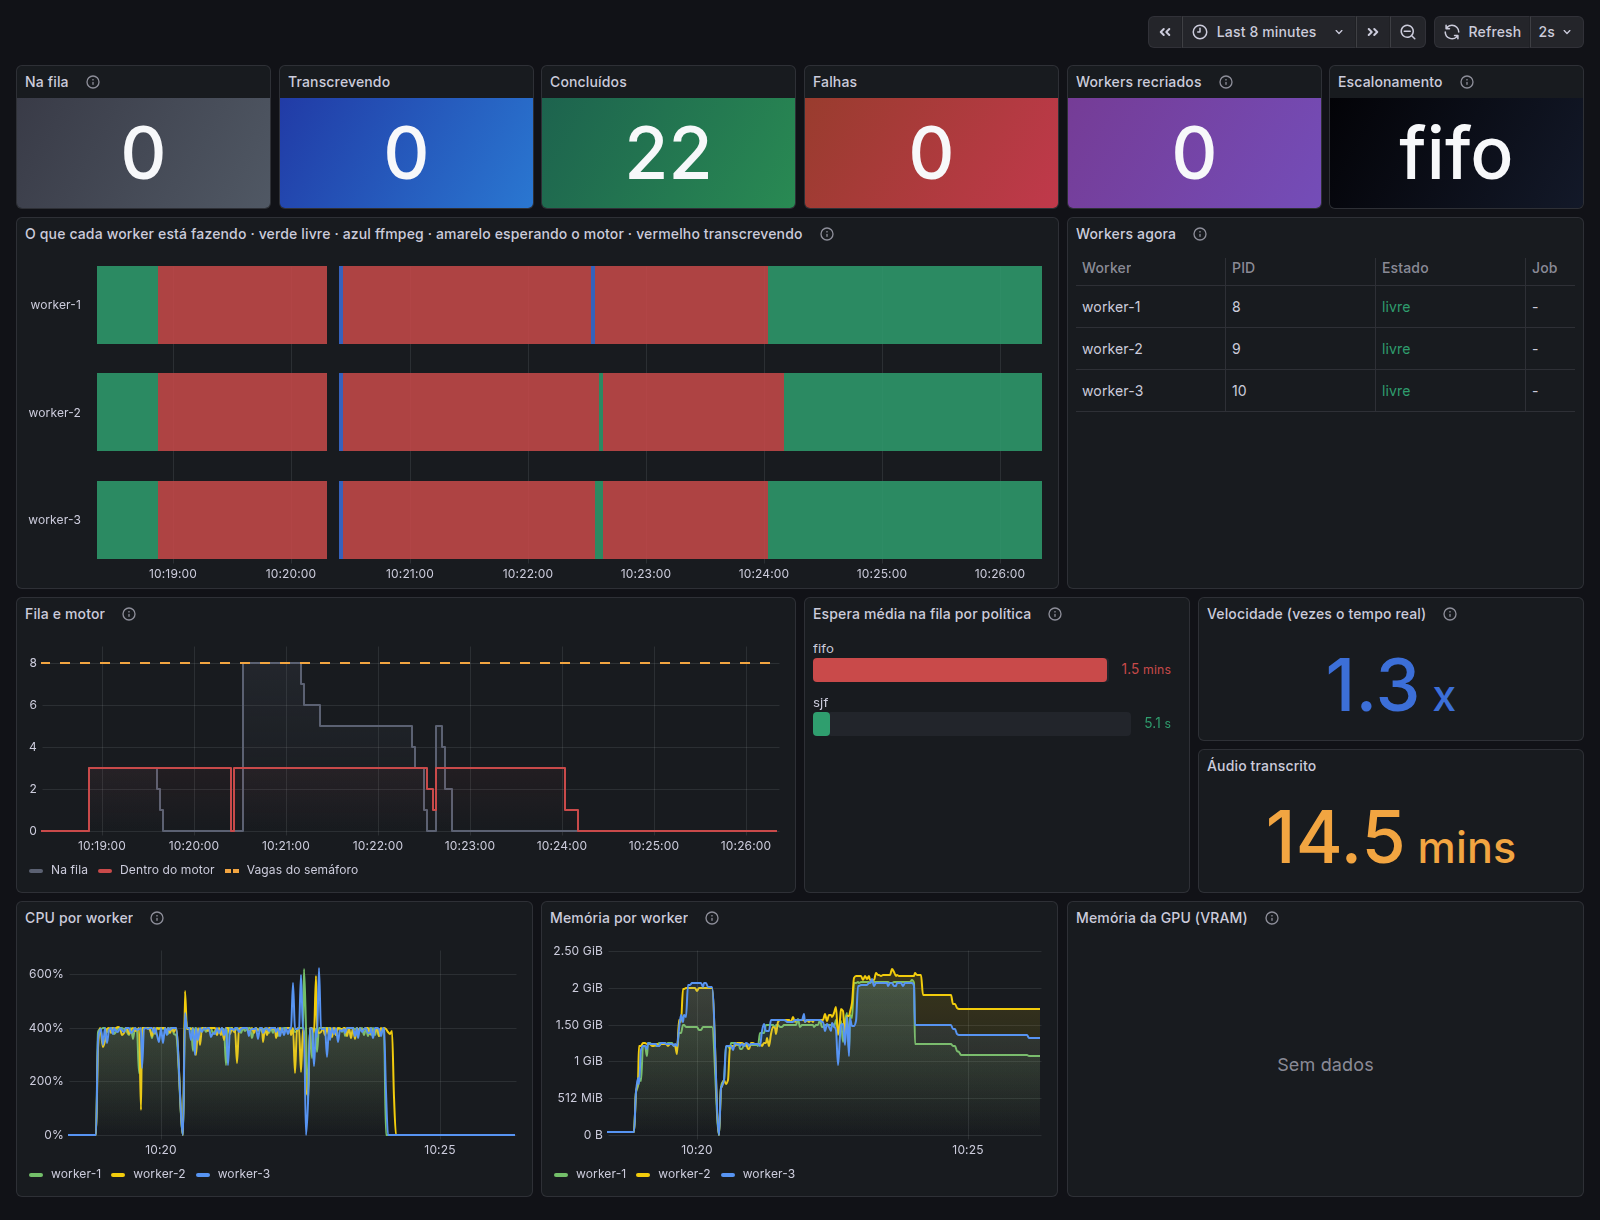
\includegraphics[width=\textwidth]{figuras/grafana.png}
  \caption{Painel do Grafana durante a demonstração de escalonamento}
  \label{fig:grafana}
\end{figure}

% ========== 5. TESTES ==========
\section{Testes e resultados}

\begin{itemize}
  \item \textbf{Testes automáticos} (\texttt{pytest}): escalonador (FIFO, SJF, devolução à fila),
        formatos TXT e SRT, escolha dos modelos por memória e recuperação da fila no banco.
        Rodam a cada envio no GitHub Actions.
  \item \textbf{Concorrência}: seis áudios de um minuto com três \emph{workers}; cada um processou
        dois, nenhum trabalho foi pego duas vezes, e o semáforo deixou um por vez na GPU.
  \item \textbf{Falha}: descrito na seção de tolerância a falhas.
  \item \textbf{Escalonamento}: tabela da seção de escalonamento.
  \item \textbf{Desempenho}: na GPU (RTX 4060, modelo \emph{Turbo}), um áudio de 10 minutos levou
        de 30 a 60 segundos, conforme a carga da máquina. Na CPU (modelo \emph{Small}, quatro threads por \emph{worker}), um
        áudio de 1 minuto levou de 40 a 60 segundos com três \emph{workers} em paralelo.
\end{itemize}

\pendente{Resultado no Windows e na máquina da apresentação.}

% ========== 6. CONCLUSÃO ==========
\section{Conclusão}
\pendente{O que o grupo aprendeu sobre a relação entre o sistema operacional e a aplicação,
as limitações (por exemplo, a GPU só acelera em placas NVIDIA) e melhorias futuras.}

% ========== REFERÊNCIAS ==========
\begin{thebibliography}{9}
\bibitem{tanenbaum}
  TANENBAUM, A. S.; BOS, H. \textit{Sistemas Operacionais Modernos}. 4. ed. São Paulo: Pearson, 2016.
\bibitem{silberschatz}
  SILBERSCHATZ, A.; GALVIN, P. B.; GAGNE, G. \textit{Fundamentos de Sistemas Operacionais}. 9. ed. Rio de Janeiro: LTC, 2015.
\bibitem{whisper}
  RADFORD, A. et al. \textit{Robust Speech Recognition via Large-Scale Weak Supervision}. 2022. Disponível em: \url{https://arxiv.org/abs/2212.04356}.
\bibitem{python}
  PYTHON SOFTWARE FOUNDATION. \textit{multiprocessing --- Process-based parallelism}. Disponível em: \url{https://docs.python.org/3/library/multiprocessing.html}.
\bibitem{docker}
  DOCKER INC. \textit{Docker Documentation}. Disponível em: \url{https://docs.docker.com/}.
\end{thebibliography}

\end{document}
